\documentclass{article}[18pt]
\usepackage{../../../../format}
\lhead{Software Methodologies - Image Processing}


\begin{document}
\begin{center}
\underline{\huge Images in Fourier Representation - Fourier Space I}
\end{center}
\section{Summary}
The Fourier transform of an image is a global transform\\
\\
Produces a representation of the image in Fourier space, (or frequency domain where there is no room for ambiguity as to the type of transform that was used)\\
\\
Performed in images by applying the Discrete Fourier Transform (DFT) operator\\
\\
Discrete Fourier Transform:
\begin{itemize}
	\item Decomposes image into frequency components (sinusoidal functions)
	\item Typically. the frequency components are arranged in array the same size as the image (sometimes it is convenient to think of the output of the DFT as an image, even though the 'pixel values' are complex numbers)
	\item Major applications in image processing, analysis and compression
\end{itemize}
\section{Terminology}
\begin{defin}[Spatial domain (or real domain, or real space)]
Images (signals) are represented by a spatial layour of the samples that are real numbers
\end{defin}

\begin{defin}[Frequency domain (or Fourier domain, or frequency/Fourier space)]
Images (signals) are represented by coefficients of sinusoidal basis frequencies  
\end{defin}
\section{1D Fourier series}
Our building block
$$A\cdot \sin(\omega \cdot x + \varphi)$$
Add enough of them to get any signal
$$f(x)=f_1(x)+f_2(x)+f_3(x)+\ldots$$
$\omega$ is the frequency. For each frequency we have one sinusoidal function in the sum.\\
\\
A is the amplitude. It is the weight of that sinusoidal function in the sum\\
\\
$\varphi$ is the phase. Changes in the phase shift a sinusoidal function left or right
\begin{center}
	\includegraphics[scale=0.7]{"1D Fourier"}
\end{center}
Low frequency components influence the coarse outline of the signal\\
\\
Higher frequency components influence the fine detail of the signal\\
\\
As we increase the number of frequency components the later, higher frequency components contribute less to the coarse outline of the signal and more to the fine detail of its shape
\section{Fourier transform}
We want to understand the signal as a sum of weighted and phase shifted frequencies. The Fourier transform reparametrises the signal by $\omega$ instead of x
\begin{center}
	\includegraphics[scale=0.7]{"fourier transform"}
\end{center}
$F(\omega)$ itself is called the Fourier transform of $f(x)$. The inverse Fourier transform applied on $F(\omega)$ parametrizes the signal again by x
\section{1D discrete Fourier transform}
The Fourier transform $M * f(x)=f(\omega)$ is a change of mathematical basis\\
\\
M: set of basis functions (N samples from each sinusoidal function form one row of the $N\times N$ matrix)\\
\\
$f(x)$: spatial domain representation (N samples of a signal arranged as a vertical vector)\\
\\
$F(\omega)$: Fourier domain representation (N frequency coefficients arranged as a vertical vector)
\begin{center}
	\includegraphics[scale=0.7]{"1D Discrete Fourier"}
\end{center}
The inverse Fourier transform $M^{-1}*F(\omega)=f(x)$ is again a change of basis
\section{Complex numbers in Fourier transform}
For every frequency $\omega$, the Fourier transform at that point $F(\omega)$ is defined by the amplitude A and the phase $\varphi$ of the corresponding sine\\
\\
While in principle we can handle amplitude and phase separately, as two real functions, mathematically it is very convenient to use complex number
\[
\begin{array}{c}{F(\omega)=R(\omega)+i I(\omega)} \\ {A=\pm \sqrt{R(\omega)^{2}+I(\omega)^{2}}} \\ {\varphi=\tan ^{-1} \frac{I(\omega)}{R(\omega)}}\end{array}
\]
\section{1D continuous Fourier transform}
By taking integrals instead of infinite sums, we can extend the Fourier transform to continuous functions
\begin{center}
	\includegraphics[scale=0.7]{"1D Continuous Fourier"}
\end{center}
\section{2D sine functions}
Any image can be reconstructed as a weighted sum of different frequencies aligned in different phases\\
The weights are the Fourier coefficients of the image
\section{Discrete Fourier transform}
The Fourier transform operator we apply on images is called the Discrete Fourier Transform (DFT)\\
\\
Inverted by the Inverse Discrete Fourier Transform (DFT$^{-1}$)\\
\\
Why "discrete"? Because of the discrete nature of image sampling (pixels)\\
\\
Computable efficiently via Fast Fourier Transform (FFT) algorithm
\begin{itemize}
	\item 1D FFT is $\mathcal{O}(N\log_2N)$
	\item 2D FFT is a series of 2N 1D FFTs
\end{itemize}
\section{Fast Fourier Transform}
DFT admits description in terms of multiplication by the Fourier matrix\\
\\
The special structure of the DFT matrix means that the multiplication of a 1D signal (an $N\times 1$ vector) by the DFT matrix can be done faster than general matrix multiplication via the FFT algorithm
\section{Visualising Fourier images}
\begin{center}
	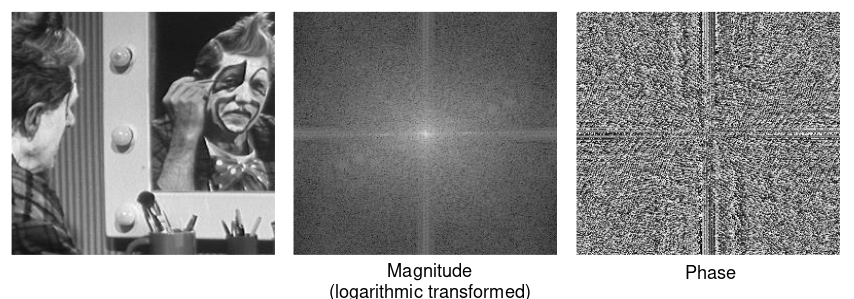
\includegraphics[scale=0.7]{visualise}
\end{center}

The output $F_{nm}$ of the DFT of an input image $I_{input}$ is a complex number valued output image containing the coefficients of the DFT of $I_{input}$\\
\\
Known as the \textbf{Fourier spectrum} of $I_{input}$, its dimension is $n\times m$ (the same as $I_{input}$)\\
\\
It can be displayed as the real and imaginary parts of the complex image
$$F_{nm}=G_{nm}+iH_{nm}$$
where
$$G_{nm} = \text{real part of} F_{nm}$$
$$H_{nm} = \text{imaginary part of} F_nm$$
Components commonly used for visualising the Fourier spectrum\\
\\
Amplitude (magnitude) spectrum
\[
\left|F_{n m}\right|=\sqrt{G_{n m}^{2}+H_{n m}^{2}}
\]
Phase spectrum:
\[
\varphi_{n m}=\tan ^{-1}\left(\frac{H_{n m}}{G_{n m}}\right)
\]
Power spectrum (where $|\cdot|$ is the norm of a complex number)
$$|F_{nm}|^2$$
The image mean intensity, which is given by the Fourier coefficient F(0,0) and is also known as the DC-component, is at the centre (by convention)\\
\\
The highest frequency present is $F(N-1,N-1)$\\
\\
The magnitude is presented on a logarithmic scale $\ln(1+|F_{nm}|)$ as the floating point range is vary large
\section{Understanding Fourier spectrum}
Magnitude and phase contain \textbf{all frequencies}\\
\\
\textbf{Lower frequencies} (close to the centre of magnitude image) are larger than the \textbf{higher frequencies} (near the boundary of the magnitude image). Thus, \textbf{more information in lower frequencies}.\\
\\
Two predominant directions in the magnitude image (horizontally and vertically correspond to patterns of the original image)\\
\\
The \textbf{phase spectrum} contains the phase part of the frequencies\\
\\
Vertical and horizontal features correspond to image patterns\\
\\
In general, the phase spectrum does not contain much structural information about the original image. However, it is crucial in reconstructing the original via inverse Fourier transform. Signal reconstruction needs phase and amplitude
\section{DFT: individual frequency components}
Removing frequencies in the Fourier domain by setting their magnitude to zero results in frequency filtering in the spatial domain.
\section{Discrete Convolution Theorem}
Convolution in the spatial domain reduces to multiplication in the frequency domain
\[
I_{A} * I_{B}=\mathrm{DFT}^{-1}\left(\mathrm{DFT}\left(I_{A}\right) \cdot \mathrm{DFT}\left(I_{B}\right)\right)
\]
Where $*$ denotes convolution of two matrices and $\cdot$ denotes component-wise multiplication of the elements of two matrices
\section{Applications of DFT}
Fourier space filtering, suppressing certain frequencies whilst leaving others unchanged\\
\\
Example:
\begin{itemize}
	\item Compute and inspect the amplitude spectrum of the image
	\item Hand-craft a binary mask P
	\begin{itemize}
		\item 1 to keep a frequency
		\item 0 to remove that frequency
	\end{itemize}
	\item Component wise multiplication of amplitude spectrum and mask P
	\item Inverse Fourier transform
\end{itemize}
JPEG compression algorithm based on a Fourier related transform called Discrete Cosine Transform (DCT)
Efficient implementation of spatial filtering:
\begin{itemize}
	\item Make image and mask the same dimension by zero padding
	\item Apply FFT to the image and to the mask
	\item Component wise multiplication of the corresponding Fourier spectra
	\item Return to the spatial domain by applying inverse FFT
\end{itemize}
If the mask is large, for example larger than $20\times 20$, the above algorithm is more efficient than doing to convolution directly in the spatial domain.\\
\\
Some image processing / computer vision libraries switch automatically to this algorithm when the mask is large.\\
\\
Using the convolution theorem, predict the behaviour of a filter against variations in the frequency of the noise\\
\\
The behaviour of the mean filter against variations in noise frequency is erratic\\
\\
The Fourier transform of a Gaussian is again a Gaussian.
\section{DFT - a few asides}
The DFT is only an approximation to the Fourier transform of the continuous image from which the digital image was obtained\\
\\
\textbf{Edge effects}: DFT assumes the digital image is one period of a periodic function (in both directions)\\
\\
If the values at the opposite edges of the function are not the same, the result is additional edge discontinuities\\
\\
\textbf{Frequency aliasing}: DFT inaccuracy from under-sampling causes frequency aliasing 

\end{document}